\documentclass[twoside]{book}

% Packages required by doxygen
\usepackage{fixltx2e}
\usepackage{calc}
\usepackage{doxygen}
\usepackage[export]{adjustbox} % also loads graphicx
\usepackage{graphicx}
\usepackage[utf8]{inputenc}
\usepackage{makeidx}
\usepackage{multicol}
\usepackage{multirow}
\PassOptionsToPackage{warn}{textcomp}
\usepackage{textcomp}
\usepackage[nointegrals]{wasysym}
\usepackage[table]{xcolor}

% Font selection
\usepackage[T1]{fontenc}
\usepackage[scaled=.90]{helvet}
\usepackage{courier}
\usepackage{amssymb}
\usepackage{sectsty}
\renewcommand{\familydefault}{\sfdefault}
\allsectionsfont{%
  \fontseries{bc}\selectfont%
  \color{darkgray}%
}
\renewcommand{\DoxyLabelFont}{%
  \fontseries{bc}\selectfont%
  \color{darkgray}%
}
\newcommand{\+}{\discretionary{\mbox{\scriptsize$\hookleftarrow$}}{}{}}

% Page & text layout
\usepackage{geometry}
\geometry{%
  a4paper,%
  top=2.5cm,%
  bottom=2.5cm,%
  left=2.5cm,%
  right=2.5cm%
}
\tolerance=750
\hfuzz=15pt
\hbadness=750
\setlength{\emergencystretch}{15pt}
\setlength{\parindent}{0cm}
\setlength{\parskip}{3ex plus 2ex minus 2ex}
\makeatletter
\renewcommand{\paragraph}{%
  \@startsection{paragraph}{4}{0ex}{-1.0ex}{1.0ex}{%
    \normalfont\normalsize\bfseries\SS@parafont%
  }%
}
\renewcommand{\subparagraph}{%
  \@startsection{subparagraph}{5}{0ex}{-1.0ex}{1.0ex}{%
    \normalfont\normalsize\bfseries\SS@subparafont%
  }%
}
\makeatother

% Headers & footers
\usepackage{fancyhdr}
\pagestyle{fancyplain}
\fancyhead[LE]{\fancyplain{}{\bfseries\thepage}}
\fancyhead[CE]{\fancyplain{}{}}
\fancyhead[RE]{\fancyplain{}{\bfseries\leftmark}}
\fancyhead[LO]{\fancyplain{}{\bfseries\rightmark}}
\fancyhead[CO]{\fancyplain{}{}}
\fancyhead[RO]{\fancyplain{}{\bfseries\thepage}}
\fancyfoot[LE]{\fancyplain{}{}}
\fancyfoot[CE]{\fancyplain{}{}}
\fancyfoot[RE]{\fancyplain{}{\bfseries\scriptsize Generated by Doxygen }}
\fancyfoot[LO]{\fancyplain{}{\bfseries\scriptsize Generated by Doxygen }}
\fancyfoot[CO]{\fancyplain{}{}}
\fancyfoot[RO]{\fancyplain{}{}}
\renewcommand{\footrulewidth}{0.4pt}
\renewcommand{\chaptermark}[1]{%
  \markboth{#1}{}%
}
\renewcommand{\sectionmark}[1]{%
  \markright{\thesection\ #1}%
}

% Indices & bibliography
\usepackage{natbib}
\usepackage[titles]{tocloft}
\setcounter{tocdepth}{3}
\setcounter{secnumdepth}{5}
\makeindex

% Hyperlinks (required, but should be loaded last)
\usepackage{ifpdf}
\ifpdf
  \usepackage[pdftex,pagebackref=true]{hyperref}
\else
  \usepackage[ps2pdf,pagebackref=true]{hyperref}
\fi
\hypersetup{%
  colorlinks=true,%
  linkcolor=blue,%
  citecolor=blue,%
  unicode%
}

% Custom commands
\newcommand{\clearemptydoublepage}{%
  \newpage{\pagestyle{empty}\cleardoublepage}%
}

\usepackage{caption}
\captionsetup{labelsep=space,justification=centering,font={bf},singlelinecheck=off,skip=4pt,position=top}

%===== C O N T E N T S =====

\begin{document}

% Titlepage & ToC
\hypersetup{pageanchor=false,
             bookmarksnumbered=true,
             pdfencoding=unicode
            }
\pagenumbering{roman}
\begin{titlepage}
\vspace*{7cm}
\begin{center}%
{\Large My Project }\\
\vspace*{1cm}
{\large Generated by Doxygen 1.8.11}\\
\end{center}
\end{titlepage}
\clearemptydoublepage
\tableofcontents
\clearemptydoublepage
\pagenumbering{arabic}
\hypersetup{pageanchor=true}

%--- Begin generated contents ---
\chapter{Class Index}
\section{Class List}
Here are the classes, structs, unions and interfaces with brief descriptions\+:\begin{DoxyCompactList}
\item\contentsline{section}{\hyperlink{structnode}{node} }{\pageref{structnode}}{}
\item\contentsline{section}{\hyperlink{structnode1}{node1} }{\pageref{structnode1}}{}
\item\contentsline{section}{\hyperlink{structnode__info}{node\+\_\+info} }{\pageref{structnode__info}}{}
\end{DoxyCompactList}

\chapter{File Index}
\section{File List}
Here is a list of all files with brief descriptions\+:\begin{DoxyCompactList}
\item\contentsline{section}{\hyperlink{Lab1_8c}{Lab1.\+c} }{\pageref{Lab1_8c}}{}
\end{DoxyCompactList}

\chapter{Class Documentation}
\hypertarget{classBinomialHeap}{}\section{Binomial\+Heap Class Reference}
\label{classBinomialHeap}\index{Binomial\+Heap@{Binomial\+Heap}}


Collaboration diagram for Binomial\+Heap\+:
\nopagebreak
\begin{figure}[H]
\begin{center}
\leavevmode
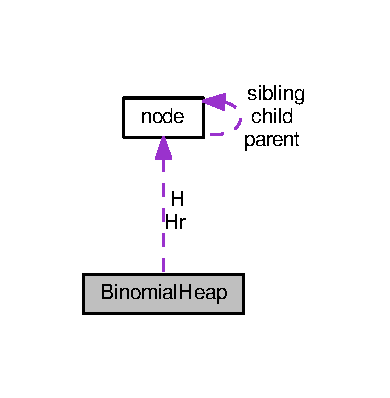
\includegraphics[width=187pt]{classBinomialHeap__coll__graph}
\end{center}
\end{figure}
\subsection*{Public Member Functions}
\begin{DoxyCompactItemize}
\item 
\hyperlink{structnode}{node} $\ast$ \hyperlink{classBinomialHeap_a3ffaab6756189d14dd76e4e7a48147b6}{Initializeheap} ()
\item 
int \hyperlink{classBinomialHeap_a657d892542f95da35f386fbe35564a35}{Binomial\+\_\+link} (\hyperlink{structnode}{node} $\ast$, \hyperlink{structnode}{node} $\ast$)
\item 
\hyperlink{structnode}{node} $\ast$ \hyperlink{classBinomialHeap_a60a7f08bad4dd38fe2b3000d6e29724e}{Create\+\_\+node} (int)
\item 
\hyperlink{structnode}{node} $\ast$ \hyperlink{classBinomialHeap_aea4c422323bcafcedb9168c86adadfa8}{Union} (\hyperlink{structnode}{node} $\ast$, \hyperlink{structnode}{node} $\ast$)
\item 
\hyperlink{structnode}{node} $\ast$ \hyperlink{classBinomialHeap_a762a7e29d6bea85540f1a82cbca4a062}{Insert} (\hyperlink{structnode}{node} $\ast$, \hyperlink{structnode}{node} $\ast$)
\item 
\hyperlink{structnode}{node} $\ast$ \hyperlink{classBinomialHeap_ade996e0273f3fcfa92b4dcce69ed111b}{Merge} (\hyperlink{structnode}{node} $\ast$, \hyperlink{structnode}{node} $\ast$)
\item 
\hyperlink{structnode}{node} $\ast$ \hyperlink{classBinomialHeap_a71e1468e2782db3f2322d188bca1e48a}{Extract\+\_\+\+Min} (\hyperlink{structnode}{node} $\ast$)
\item 
int \hyperlink{classBinomialHeap_a59481a0ec3750711c68e9ddd21443707}{Revert\+\_\+list} (\hyperlink{structnode}{node} $\ast$)
\item 
int \hyperlink{classBinomialHeap_a43b3339eb8cc6eea26f769ab616b720a}{Display} (\hyperlink{structnode}{node} $\ast$)
\item 
\hyperlink{structnode}{node} $\ast$ \hyperlink{classBinomialHeap_a5066787434a932210311500f671d2202}{Search} (\hyperlink{structnode}{node} $\ast$, int)
\item 
int \hyperlink{classBinomialHeap_a3898a1fb87677fdb94a40f62ac416de9}{Decrease\+\_\+key} (\hyperlink{structnode}{node} $\ast$, int, int)
\item 
int \hyperlink{classBinomialHeap_aab7ea7e42fe1b2aaf3298f73f4e68884}{Delete} (\hyperlink{structnode}{node} $\ast$, int)
\item 
\hyperlink{classBinomialHeap_ace4f32509eae5e8508433d7e291f2a3e}{Binomial\+Heap} ()
\end{DoxyCompactItemize}
\subsection*{Private Attributes}
\begin{DoxyCompactItemize}
\item 
\hyperlink{structnode}{node} $\ast$ \hyperlink{classBinomialHeap_acf5c4a0779ec8b4306776a525620c5b1}{H}
\item 
\hyperlink{structnode}{node} $\ast$ \hyperlink{classBinomialHeap_ac1d71f6b98b604dda25fcfcca53cc071}{Hr}
\item 
int \hyperlink{classBinomialHeap_ade4b936fdd0d31cf3879cac08b44f38c}{count}
\end{DoxyCompactItemize}


\subsection{Constructor \& Destructor Documentation}
\index{Binomial\+Heap@{Binomial\+Heap}!Binomial\+Heap@{Binomial\+Heap}}
\index{Binomial\+Heap@{Binomial\+Heap}!Binomial\+Heap@{Binomial\+Heap}}
\subsubsection[{\texorpdfstring{Binomial\+Heap()}{BinomialHeap()}}]{\setlength{\rightskip}{0pt plus 5cm}Binomial\+Heap\+::\+Binomial\+Heap (
\begin{DoxyParamCaption}
{}
\end{DoxyParamCaption}
)\hspace{0.3cm}{\ttfamily [inline]}}\hypertarget{classBinomialHeap_ace4f32509eae5e8508433d7e291f2a3e}{}\label{classBinomialHeap_ace4f32509eae5e8508433d7e291f2a3e}

\begin{DoxyCode}
41         \{
42             \hyperlink{classBinomialHeap_acf5c4a0779ec8b4306776a525620c5b1}{H} = \hyperlink{classBinomialHeap_a3ffaab6756189d14dd76e4e7a48147b6}{Initializeheap}();
43             \hyperlink{classBinomialHeap_ac1d71f6b98b604dda25fcfcca53cc071}{Hr} = \hyperlink{classBinomialHeap_a3ffaab6756189d14dd76e4e7a48147b6}{Initializeheap}();
44             \textcolor{keywordtype}{int} \hyperlink{classBinomialHeap_ade4b936fdd0d31cf3879cac08b44f38c}{count} = 1;
45         \}
\end{DoxyCode}


\subsection{Member Function Documentation}
\index{Binomial\+Heap@{Binomial\+Heap}!Binomial\+\_\+link@{Binomial\+\_\+link}}
\index{Binomial\+\_\+link@{Binomial\+\_\+link}!Binomial\+Heap@{Binomial\+Heap}}
\subsubsection[{\texorpdfstring{Binomial\+\_\+link(node $\ast$, node $\ast$)}{Binomial_link(node *, node *)}}]{\setlength{\rightskip}{0pt plus 5cm}int Binomial\+Heap\+::\+Binomial\+\_\+link (
\begin{DoxyParamCaption}
\item[{{\bf node} $\ast$}]{y, }
\item[{{\bf node} $\ast$}]{z}
\end{DoxyParamCaption}
)}\hypertarget{classBinomialHeap_a657d892542f95da35f386fbe35564a35}{}\label{classBinomialHeap_a657d892542f95da35f386fbe35564a35}

\begin{DoxyCode}
61 \{
62     y->\hyperlink{structnode_a5e88137f1d0e2f7a940bccf4c3d3a4d3}{parent} = z;
63     y->\hyperlink{structnode_a0941f5cd2e8bd7fda70619bb099f267d}{sibling} = z->\hyperlink{structnode_a422bd5292acd3b746c3f3113f76de9a7}{child};
64     z->\hyperlink{structnode_a422bd5292acd3b746c3f3113f76de9a7}{child} = y;
65     z->\hyperlink{structnode_a5ef19e24e48768739e8743eccbc81434}{degree} = z->\hyperlink{structnode_a5ef19e24e48768739e8743eccbc81434}{degree} + 1;
66 \}
\end{DoxyCode}
\index{Binomial\+Heap@{Binomial\+Heap}!Create\+\_\+node@{Create\+\_\+node}}
\index{Create\+\_\+node@{Create\+\_\+node}!Binomial\+Heap@{Binomial\+Heap}}
\subsubsection[{\texorpdfstring{Create\+\_\+node(int)}{Create_node(int)}}]{\setlength{\rightskip}{0pt plus 5cm}{\bf node} $\ast$ Binomial\+Heap\+::\+Create\+\_\+node (
\begin{DoxyParamCaption}
\item[{int}]{k}
\end{DoxyParamCaption}
)}\hypertarget{classBinomialHeap_a60a7f08bad4dd38fe2b3000d6e29724e}{}\label{classBinomialHeap_a60a7f08bad4dd38fe2b3000d6e29724e}

\begin{DoxyCode}
71 \{
72     \hyperlink{structnode}{node}* p = \textcolor{keyword}{new} \hyperlink{structnode}{node};
73     p->\hyperlink{structnode_a027ad0e5186d6cfab02c74a3da2d28a9}{n} = k;
74     \textcolor{keywordflow}{return} p;
75 \}
\end{DoxyCode}
\index{Binomial\+Heap@{Binomial\+Heap}!Decrease\+\_\+key@{Decrease\+\_\+key}}
\index{Decrease\+\_\+key@{Decrease\+\_\+key}!Binomial\+Heap@{Binomial\+Heap}}
\subsubsection[{\texorpdfstring{Decrease\+\_\+key(node $\ast$, int, int)}{Decrease_key(node *, int, int)}}]{\setlength{\rightskip}{0pt plus 5cm}int Binomial\+Heap\+::\+Decrease\+\_\+key (
\begin{DoxyParamCaption}
\item[{{\bf node} $\ast$}]{H, }
\item[{int}]{i, }
\item[{int}]{k}
\end{DoxyParamCaption}
)}\hypertarget{classBinomialHeap_a3898a1fb87677fdb94a40f62ac416de9}{}\label{classBinomialHeap_a3898a1fb87677fdb94a40f62ac416de9}

\begin{DoxyCode}
283 \{
284     \textcolor{keywordtype}{int} temp;
285     \hyperlink{structnode}{node}* p;
286     \hyperlink{structnode}{node}* y;
287     \hyperlink{structnode}{node}* z;
288     p = \hyperlink{classBinomialHeap_a5066787434a932210311500f671d2202}{Search}(H, i);
289     \textcolor{keywordflow}{if} (p == NULL)
290     \{
291         cout<<\textcolor{stringliteral}{"Invalid choice of key"}<<endl;
292         \textcolor{keywordflow}{return} 0;
293     \}
294     \textcolor{keywordflow}{if} (k > p->\hyperlink{structnode_a027ad0e5186d6cfab02c74a3da2d28a9}{n})
295     \{
296         cout<<\textcolor{stringliteral}{"Error!! New key is greater than current key"}<<endl;
297         \textcolor{keywordflow}{return} 0;
298     \}
299     p->\hyperlink{structnode_a027ad0e5186d6cfab02c74a3da2d28a9}{n} = k;
300     y = p;
301     z = p->\hyperlink{structnode_a5e88137f1d0e2f7a940bccf4c3d3a4d3}{parent};
302     \textcolor{keywordflow}{while} (z != NULL && y->\hyperlink{structnode_a027ad0e5186d6cfab02c74a3da2d28a9}{n} < z->\hyperlink{structnode_a027ad0e5186d6cfab02c74a3da2d28a9}{n})
303     \{
304         temp = y->\hyperlink{structnode_a027ad0e5186d6cfab02c74a3da2d28a9}{n};
305         y->\hyperlink{structnode_a027ad0e5186d6cfab02c74a3da2d28a9}{n} = z->\hyperlink{structnode_a027ad0e5186d6cfab02c74a3da2d28a9}{n};
306         z->\hyperlink{structnode_a027ad0e5186d6cfab02c74a3da2d28a9}{n} = temp;
307         y = z;
308         z = z->\hyperlink{structnode_a5e88137f1d0e2f7a940bccf4c3d3a4d3}{parent};
309     \}
310     cout<<\textcolor{stringliteral}{"Key reduced successfully"}<<endl;
311 \}
\end{DoxyCode}
\index{Binomial\+Heap@{Binomial\+Heap}!Delete@{Delete}}
\index{Delete@{Delete}!Binomial\+Heap@{Binomial\+Heap}}
\subsubsection[{\texorpdfstring{Delete(node $\ast$, int)}{Delete(node *, int)}}]{\setlength{\rightskip}{0pt plus 5cm}int Binomial\+Heap\+::\+Delete (
\begin{DoxyParamCaption}
\item[{{\bf node} $\ast$}]{H, }
\item[{int}]{k}
\end{DoxyParamCaption}
)}\hypertarget{classBinomialHeap_aab7ea7e42fe1b2aaf3298f73f4e68884}{}\label{classBinomialHeap_aab7ea7e42fe1b2aaf3298f73f4e68884}

\begin{DoxyCode}
316 \{
317     \hyperlink{structnode}{node}* np;
318     \textcolor{keywordflow}{if} (H == NULL)
319     \{
320         cout<<\textcolor{stringliteral}{"\(\backslash\)nHEAP EMPTY!!!!!"};
321         \textcolor{keywordflow}{return} 0;
322     \}
323     \hyperlink{classBinomialHeap_a3898a1fb87677fdb94a40f62ac416de9}{Decrease\_key}(H, k, -1000);
324     np = \hyperlink{classBinomialHeap_a71e1468e2782db3f2322d188bca1e48a}{Extract\_Min}(H);
325     \textcolor{keywordflow}{if} (np != NULL)
326         cout<<\textcolor{stringliteral}{"Node Deleted Successfully"}<<endl;
327 \}
\end{DoxyCode}
\index{Binomial\+Heap@{Binomial\+Heap}!Display@{Display}}
\index{Display@{Display}!Binomial\+Heap@{Binomial\+Heap}}
\subsubsection[{\texorpdfstring{Display(node $\ast$)}{Display(node *)}}]{\setlength{\rightskip}{0pt plus 5cm}int Binomial\+Heap\+::\+Display (
\begin{DoxyParamCaption}
\item[{{\bf node} $\ast$}]{H}
\end{DoxyParamCaption}
)}\hypertarget{classBinomialHeap_a43b3339eb8cc6eea26f769ab616b720a}{}\label{classBinomialHeap_a43b3339eb8cc6eea26f769ab616b720a}

\begin{DoxyCode}
186 \{
187     \textcolor{keywordflow}{if} (H == NULL)
188     \{
189         cout<<\textcolor{stringliteral}{"The Heap is empty"}<<endl;
190         \textcolor{keywordflow}{return} 0;
191     \}
192     cout<<\textcolor{stringliteral}{"The root nodes are: "}<<endl;
193     \hyperlink{structnode}{node}* p;
194     p = \hyperlink{classBinomialHeap_acf5c4a0779ec8b4306776a525620c5b1}{H};
195     \textcolor{keywordflow}{while} (p != NULL)
196     \{
197         cout<<p->\hyperlink{structnode_a027ad0e5186d6cfab02c74a3da2d28a9}{n};
198         \textcolor{keywordflow}{if} (p->\hyperlink{structnode_a0941f5cd2e8bd7fda70619bb099f267d}{sibling} != NULL)
199             cout<<\textcolor{stringliteral}{"-->"};
200         p = p->\hyperlink{structnode_a0941f5cd2e8bd7fda70619bb099f267d}{sibling};
201     \}
202     cout<<endl;
203 \}
\end{DoxyCode}
\index{Binomial\+Heap@{Binomial\+Heap}!Extract\+\_\+\+Min@{Extract\+\_\+\+Min}}
\index{Extract\+\_\+\+Min@{Extract\+\_\+\+Min}!Binomial\+Heap@{Binomial\+Heap}}
\subsubsection[{\texorpdfstring{Extract\+\_\+\+Min(node $\ast$)}{Extract_Min(node *)}}]{\setlength{\rightskip}{0pt plus 5cm}{\bf node} $\ast$ Binomial\+Heap\+::\+Extract\+\_\+\+Min (
\begin{DoxyParamCaption}
\item[{{\bf node} $\ast$}]{H1}
\end{DoxyParamCaption}
)}\hypertarget{classBinomialHeap_a71e1468e2782db3f2322d188bca1e48a}{}\label{classBinomialHeap_a71e1468e2782db3f2322d188bca1e48a}

\begin{DoxyCode}
208 \{
209     \hyperlink{classBinomialHeap_ac1d71f6b98b604dda25fcfcca53cc071}{Hr} = NULL;
210     \hyperlink{structnode}{node}* t = NULL;
211     \hyperlink{structnode}{node}* x = H1;
212     \textcolor{keywordflow}{if} (x == NULL)
213     \{
214         cout<<\textcolor{stringliteral}{"Nothing to Extract"}<<endl;
215         \textcolor{keywordflow}{return} x;
216     \}
217     \textcolor{keywordtype}{int} min = x->\hyperlink{structnode_a027ad0e5186d6cfab02c74a3da2d28a9}{n};
218     \hyperlink{structnode}{node}* p = x;
219     \textcolor{keywordflow}{while} (p->\hyperlink{structnode_a0941f5cd2e8bd7fda70619bb099f267d}{sibling} != NULL)
220     \{
221         \textcolor{keywordflow}{if} ((p->\hyperlink{structnode_a0941f5cd2e8bd7fda70619bb099f267d}{sibling})->n < min)
222         \{
223             min = (p->\hyperlink{structnode_a0941f5cd2e8bd7fda70619bb099f267d}{sibling})->n;
224             t = p;
225             x = p->\hyperlink{structnode_a0941f5cd2e8bd7fda70619bb099f267d}{sibling};
226         \}
227         p = p->\hyperlink{structnode_a0941f5cd2e8bd7fda70619bb099f267d}{sibling};
228     \}
229     \textcolor{keywordflow}{if} (t == NULL && x->\hyperlink{structnode_a0941f5cd2e8bd7fda70619bb099f267d}{sibling} == NULL)
230         H1 = NULL;
231     \textcolor{keywordflow}{else} \textcolor{keywordflow}{if} (t == NULL)
232         H1 = x->\hyperlink{structnode_a0941f5cd2e8bd7fda70619bb099f267d}{sibling};
233     \textcolor{keywordflow}{else} \textcolor{keywordflow}{if} (t->\hyperlink{structnode_a0941f5cd2e8bd7fda70619bb099f267d}{sibling} == NULL)
234         t = NULL;
235     \textcolor{keywordflow}{else}
236         t->\hyperlink{structnode_a0941f5cd2e8bd7fda70619bb099f267d}{sibling} = x->\hyperlink{structnode_a0941f5cd2e8bd7fda70619bb099f267d}{sibling};
237     \textcolor{keywordflow}{if} (x->\hyperlink{structnode_a422bd5292acd3b746c3f3113f76de9a7}{child} != NULL)
238     \{
239         \hyperlink{classBinomialHeap_a59481a0ec3750711c68e9ddd21443707}{Revert\_list}(x->\hyperlink{structnode_a422bd5292acd3b746c3f3113f76de9a7}{child});
240         (x->\hyperlink{structnode_a422bd5292acd3b746c3f3113f76de9a7}{child})->sibling = NULL;
241     \}
242     \hyperlink{classBinomialHeap_acf5c4a0779ec8b4306776a525620c5b1}{H} = \hyperlink{classBinomialHeap_aea4c422323bcafcedb9168c86adadfa8}{Union}(H1, \hyperlink{classBinomialHeap_ac1d71f6b98b604dda25fcfcca53cc071}{Hr});
243     \textcolor{keywordflow}{return} x;
244 \}
\end{DoxyCode}
\index{Binomial\+Heap@{Binomial\+Heap}!Initializeheap@{Initializeheap}}
\index{Initializeheap@{Initializeheap}!Binomial\+Heap@{Binomial\+Heap}}
\subsubsection[{\texorpdfstring{Initializeheap()}{Initializeheap()}}]{\setlength{\rightskip}{0pt plus 5cm}{\bf node} $\ast$ Binomial\+Heap\+::\+Initializeheap (
\begin{DoxyParamCaption}
{}
\end{DoxyParamCaption}
)}\hypertarget{classBinomialHeap_a3ffaab6756189d14dd76e4e7a48147b6}{}\label{classBinomialHeap_a3ffaab6756189d14dd76e4e7a48147b6}

\begin{DoxyCode}
52 \{
53     \hyperlink{structnode}{node}* np;
54     np = NULL;
55     \textcolor{keywordflow}{return} np;
56 \}
\end{DoxyCode}
\index{Binomial\+Heap@{Binomial\+Heap}!Insert@{Insert}}
\index{Insert@{Insert}!Binomial\+Heap@{Binomial\+Heap}}
\subsubsection[{\texorpdfstring{Insert(node $\ast$, node $\ast$)}{Insert(node *, node *)}}]{\setlength{\rightskip}{0pt plus 5cm}{\bf node} $\ast$ Binomial\+Heap\+::\+Insert (
\begin{DoxyParamCaption}
\item[{{\bf node} $\ast$}]{H, }
\item[{{\bf node} $\ast$}]{x}
\end{DoxyParamCaption}
)}\hypertarget{classBinomialHeap_a762a7e29d6bea85540f1a82cbca4a062}{}\label{classBinomialHeap_a762a7e29d6bea85540f1a82cbca4a062}

\begin{DoxyCode}
80 \{
81     \hyperlink{structnode}{node}* H1 = \hyperlink{classBinomialHeap_a3ffaab6756189d14dd76e4e7a48147b6}{Initializeheap}();
82     x->\hyperlink{structnode_a5e88137f1d0e2f7a940bccf4c3d3a4d3}{parent} = NULL;
83     x->\hyperlink{structnode_a422bd5292acd3b746c3f3113f76de9a7}{child} = NULL;
84     x->\hyperlink{structnode_a0941f5cd2e8bd7fda70619bb099f267d}{sibling} = NULL;
85     x->\hyperlink{structnode_a5ef19e24e48768739e8743eccbc81434}{degree} = 0;
86     H1 = x;
87     H = \hyperlink{classBinomialHeap_aea4c422323bcafcedb9168c86adadfa8}{Union}(H, H1);
88     \textcolor{keywordflow}{return} \hyperlink{classBinomialHeap_acf5c4a0779ec8b4306776a525620c5b1}{H};
89 \}
\end{DoxyCode}
\index{Binomial\+Heap@{Binomial\+Heap}!Merge@{Merge}}
\index{Merge@{Merge}!Binomial\+Heap@{Binomial\+Heap}}
\subsubsection[{\texorpdfstring{Merge(node $\ast$, node $\ast$)}{Merge(node *, node *)}}]{\setlength{\rightskip}{0pt plus 5cm}{\bf node} $\ast$ Binomial\+Heap\+::\+Merge (
\begin{DoxyParamCaption}
\item[{{\bf node} $\ast$}]{H1, }
\item[{{\bf node} $\ast$}]{H2}
\end{DoxyParamCaption}
)}\hypertarget{classBinomialHeap_ade996e0273f3fcfa92b4dcce69ed111b}{}\label{classBinomialHeap_ade996e0273f3fcfa92b4dcce69ed111b}

\begin{DoxyCode}
139 \{
140     \hyperlink{structnode}{node}* \hyperlink{classBinomialHeap_acf5c4a0779ec8b4306776a525620c5b1}{H} = \hyperlink{classBinomialHeap_a3ffaab6756189d14dd76e4e7a48147b6}{Initializeheap}();
141     \hyperlink{structnode}{node}* y;
142     \hyperlink{structnode}{node}* z;
143     \hyperlink{structnode}{node}* a;
144     \hyperlink{structnode}{node}* b;
145     y = H1;
146     z = H2;
147     \textcolor{keywordflow}{if} (y != NULL)
148     \{
149         \textcolor{keywordflow}{if} (z != NULL)
150         \{
151             \textcolor{keywordflow}{if} (y->\hyperlink{structnode_a5ef19e24e48768739e8743eccbc81434}{degree} <= z->\hyperlink{structnode_a5ef19e24e48768739e8743eccbc81434}{degree})
152                 H = y;
153             \textcolor{keywordflow}{else} \textcolor{keywordflow}{if} (y->\hyperlink{structnode_a5ef19e24e48768739e8743eccbc81434}{degree} > z->\hyperlink{structnode_a5ef19e24e48768739e8743eccbc81434}{degree})
154                 H = z;
155         \}
156         \textcolor{keywordflow}{else}
157             H = y;
158     \}
159     \textcolor{keywordflow}{else}
160         H = z;
161     \textcolor{keywordflow}{while} (y != NULL && z != NULL)
162     \{
163         \textcolor{keywordflow}{if} (y->\hyperlink{structnode_a5ef19e24e48768739e8743eccbc81434}{degree} < z->\hyperlink{structnode_a5ef19e24e48768739e8743eccbc81434}{degree})
164         \{
165             y = y->\hyperlink{structnode_a0941f5cd2e8bd7fda70619bb099f267d}{sibling};
166         \}
167         \textcolor{keywordflow}{else} \textcolor{keywordflow}{if} (y->\hyperlink{structnode_a5ef19e24e48768739e8743eccbc81434}{degree} == z->\hyperlink{structnode_a5ef19e24e48768739e8743eccbc81434}{degree})
168         \{
169             a = y->\hyperlink{structnode_a0941f5cd2e8bd7fda70619bb099f267d}{sibling};
170             y->\hyperlink{structnode_a0941f5cd2e8bd7fda70619bb099f267d}{sibling} = z;
171             y = a;
172         \}
173         \textcolor{keywordflow}{else}
174         \{
175             b = z->\hyperlink{structnode_a0941f5cd2e8bd7fda70619bb099f267d}{sibling};
176             z->\hyperlink{structnode_a0941f5cd2e8bd7fda70619bb099f267d}{sibling} = y;
177             z = b;
178         \}
179     \}
180     \textcolor{keywordflow}{return} \hyperlink{classBinomialHeap_acf5c4a0779ec8b4306776a525620c5b1}{H};
181 \}
\end{DoxyCode}
\index{Binomial\+Heap@{Binomial\+Heap}!Revert\+\_\+list@{Revert\+\_\+list}}
\index{Revert\+\_\+list@{Revert\+\_\+list}!Binomial\+Heap@{Binomial\+Heap}}
\subsubsection[{\texorpdfstring{Revert\+\_\+list(node $\ast$)}{Revert_list(node *)}}]{\setlength{\rightskip}{0pt plus 5cm}int Binomial\+Heap\+::\+Revert\+\_\+list (
\begin{DoxyParamCaption}
\item[{{\bf node} $\ast$}]{y}
\end{DoxyParamCaption}
)}\hypertarget{classBinomialHeap_a59481a0ec3750711c68e9ddd21443707}{}\label{classBinomialHeap_a59481a0ec3750711c68e9ddd21443707}

\begin{DoxyCode}
249 \{
250     \textcolor{keywordflow}{if} (y->\hyperlink{structnode_a0941f5cd2e8bd7fda70619bb099f267d}{sibling} != NULL)
251     \{
252         \hyperlink{classBinomialHeap_a59481a0ec3750711c68e9ddd21443707}{Revert\_list}(y->\hyperlink{structnode_a0941f5cd2e8bd7fda70619bb099f267d}{sibling});
253         (y->\hyperlink{structnode_a0941f5cd2e8bd7fda70619bb099f267d}{sibling})->sibling = y;
254     \}
255     \textcolor{keywordflow}{else}
256     \{
257         \hyperlink{classBinomialHeap_ac1d71f6b98b604dda25fcfcca53cc071}{Hr} = y;
258     \}
259 \}
\end{DoxyCode}
\index{Binomial\+Heap@{Binomial\+Heap}!Search@{Search}}
\index{Search@{Search}!Binomial\+Heap@{Binomial\+Heap}}
\subsubsection[{\texorpdfstring{Search(node $\ast$, int)}{Search(node *, int)}}]{\setlength{\rightskip}{0pt plus 5cm}{\bf node} $\ast$ Binomial\+Heap\+::\+Search (
\begin{DoxyParamCaption}
\item[{{\bf node} $\ast$}]{H, }
\item[{int}]{k}
\end{DoxyParamCaption}
)}\hypertarget{classBinomialHeap_a5066787434a932210311500f671d2202}{}\label{classBinomialHeap_a5066787434a932210311500f671d2202}

\begin{DoxyCode}
265 \{
266     \hyperlink{structnode}{node}* x = \hyperlink{classBinomialHeap_acf5c4a0779ec8b4306776a525620c5b1}{H};
267     \hyperlink{structnode}{node}* p = NULL;
268     \textcolor{keywordflow}{if} (x->\hyperlink{structnode_a027ad0e5186d6cfab02c74a3da2d28a9}{n} == k)
269     \{
270         p = x;
271         \textcolor{keywordflow}{return} p;
272     \}
273     \textcolor{keywordflow}{if} (x->\hyperlink{structnode_a422bd5292acd3b746c3f3113f76de9a7}{child} != NULL && p == NULL)
274         p = \hyperlink{classBinomialHeap_a5066787434a932210311500f671d2202}{Search}(x->\hyperlink{structnode_a422bd5292acd3b746c3f3113f76de9a7}{child}, k);
275     \textcolor{keywordflow}{if} (x->\hyperlink{structnode_a0941f5cd2e8bd7fda70619bb099f267d}{sibling} != NULL && p == NULL)
276         p = \hyperlink{classBinomialHeap_a5066787434a932210311500f671d2202}{Search}(x->\hyperlink{structnode_a0941f5cd2e8bd7fda70619bb099f267d}{sibling}, k);
277     \textcolor{keywordflow}{return} p;
278 \}
\end{DoxyCode}
\index{Binomial\+Heap@{Binomial\+Heap}!Union@{Union}}
\index{Union@{Union}!Binomial\+Heap@{Binomial\+Heap}}
\subsubsection[{\texorpdfstring{Union(node $\ast$, node $\ast$)}{Union(node *, node *)}}]{\setlength{\rightskip}{0pt plus 5cm}{\bf node} $\ast$ Binomial\+Heap\+::\+Union (
\begin{DoxyParamCaption}
\item[{{\bf node} $\ast$}]{H1, }
\item[{{\bf node} $\ast$}]{H2}
\end{DoxyParamCaption}
)}\hypertarget{classBinomialHeap_aea4c422323bcafcedb9168c86adadfa8}{}\label{classBinomialHeap_aea4c422323bcafcedb9168c86adadfa8}

\begin{DoxyCode}
95 \{
96     \hyperlink{structnode}{node} *\hyperlink{classBinomialHeap_acf5c4a0779ec8b4306776a525620c5b1}{H} = \hyperlink{classBinomialHeap_a3ffaab6756189d14dd76e4e7a48147b6}{Initializeheap}();
97     H = \hyperlink{classBinomialHeap_ade996e0273f3fcfa92b4dcce69ed111b}{Merge}(H1, H2);
98     \textcolor{keywordflow}{if} (H == NULL)
99         \textcolor{keywordflow}{return} \hyperlink{classBinomialHeap_acf5c4a0779ec8b4306776a525620c5b1}{H};
100     \hyperlink{structnode}{node}* prev\_x;
101     \hyperlink{structnode}{node}* next\_x;
102     \hyperlink{structnode}{node}* x;
103     prev\_x = NULL;
104     x = \hyperlink{classBinomialHeap_acf5c4a0779ec8b4306776a525620c5b1}{H};
105     next\_x = x->\hyperlink{structnode_a0941f5cd2e8bd7fda70619bb099f267d}{sibling};
106     \textcolor{keywordflow}{while} (next\_x != NULL)
107     \{
108         \textcolor{keywordflow}{if} ((x->\hyperlink{structnode_a5ef19e24e48768739e8743eccbc81434}{degree} != next\_x->\hyperlink{structnode_a5ef19e24e48768739e8743eccbc81434}{degree}) || ((next\_x->\hyperlink{structnode_a0941f5cd2e8bd7fda70619bb099f267d}{sibling} != NULL)
109             && (next\_x->\hyperlink{structnode_a0941f5cd2e8bd7fda70619bb099f267d}{sibling})->degree == x->\hyperlink{structnode_a5ef19e24e48768739e8743eccbc81434}{degree}))
110         \{
111             prev\_x = x;
112             x = next\_x;
113         \}
114         \textcolor{keywordflow}{else}
115         \{
116             \textcolor{keywordflow}{if} (x->\hyperlink{structnode_a027ad0e5186d6cfab02c74a3da2d28a9}{n} <= next\_x->\hyperlink{structnode_a027ad0e5186d6cfab02c74a3da2d28a9}{n})
117             \{
118                 x->\hyperlink{structnode_a0941f5cd2e8bd7fda70619bb099f267d}{sibling} = next\_x->\hyperlink{structnode_a0941f5cd2e8bd7fda70619bb099f267d}{sibling};
119                 \hyperlink{classBinomialHeap_a657d892542f95da35f386fbe35564a35}{Binomial\_link}(next\_x, x);
120             \}
121             \textcolor{keywordflow}{else}
122             \{
123                 \textcolor{keywordflow}{if} (prev\_x == NULL)
124                     H = next\_x;
125                 \textcolor{keywordflow}{else}
126                     prev\_x->\hyperlink{structnode_a0941f5cd2e8bd7fda70619bb099f267d}{sibling} = next\_x;
127                 \hyperlink{classBinomialHeap_a657d892542f95da35f386fbe35564a35}{Binomial\_link}(x, next\_x);
128                 x = next\_x;
129             \}
130         \}
131         next\_x = x->\hyperlink{structnode_a0941f5cd2e8bd7fda70619bb099f267d}{sibling};
132     \}
133     \textcolor{keywordflow}{return} \hyperlink{classBinomialHeap_acf5c4a0779ec8b4306776a525620c5b1}{H};
134 \}
\end{DoxyCode}


\subsection{Member Data Documentation}
\index{Binomial\+Heap@{Binomial\+Heap}!count@{count}}
\index{count@{count}!Binomial\+Heap@{Binomial\+Heap}}
\subsubsection[{\texorpdfstring{count}{count}}]{\setlength{\rightskip}{0pt plus 5cm}int Binomial\+Heap\+::count\hspace{0.3cm}{\ttfamily [private]}}\hypertarget{classBinomialHeap_ade4b936fdd0d31cf3879cac08b44f38c}{}\label{classBinomialHeap_ade4b936fdd0d31cf3879cac08b44f38c}
\index{Binomial\+Heap@{Binomial\+Heap}!H@{H}}
\index{H@{H}!Binomial\+Heap@{Binomial\+Heap}}
\subsubsection[{\texorpdfstring{H}{H}}]{\setlength{\rightskip}{0pt plus 5cm}{\bf node}$\ast$ Binomial\+Heap\+::H\hspace{0.3cm}{\ttfamily [private]}}\hypertarget{classBinomialHeap_acf5c4a0779ec8b4306776a525620c5b1}{}\label{classBinomialHeap_acf5c4a0779ec8b4306776a525620c5b1}
\index{Binomial\+Heap@{Binomial\+Heap}!Hr@{Hr}}
\index{Hr@{Hr}!Binomial\+Heap@{Binomial\+Heap}}
\subsubsection[{\texorpdfstring{Hr}{Hr}}]{\setlength{\rightskip}{0pt plus 5cm}{\bf node}$\ast$ Binomial\+Heap\+::\+Hr\hspace{0.3cm}{\ttfamily [private]}}\hypertarget{classBinomialHeap_ac1d71f6b98b604dda25fcfcca53cc071}{}\label{classBinomialHeap_ac1d71f6b98b604dda25fcfcca53cc071}


The documentation for this class was generated from the following file\+:\begin{DoxyCompactItemize}
\item 
\hyperlink{BinomialHeap_8cpp}{Binomial\+Heap.\+cpp}\end{DoxyCompactItemize}

\hypertarget{structnode}{}\section{node Struct Reference}
\label{structnode}\index{node@{node}}


Collaboration diagram for node\+:
\nopagebreak
\begin{figure}[H]
\begin{center}
\leavevmode
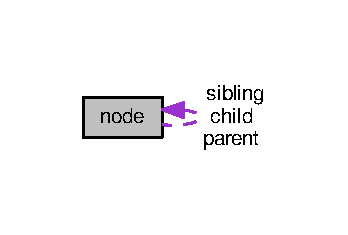
\includegraphics[width=158pt]{structnode__coll__graph}
\end{center}
\end{figure}
\subsection*{Public Attributes}
\begin{DoxyCompactItemize}
\item 
int \hyperlink{structnode_a2d890bb9f6af0ffd73fe79b21124c2a2}{data}
\item 
\hyperlink{structnode}{node} $\ast$ \hyperlink{structnode_aad210fa7c160a49f6b9a3ffee592a2bc}{next}
\end{DoxyCompactItemize}


\subsection{Member Data Documentation}
\index{node@{node}!data@{data}}
\index{data@{data}!node@{node}}
\subsubsection[{\texorpdfstring{data}{data}}]{\setlength{\rightskip}{0pt plus 5cm}int node\+::data}\hypertarget{structnode_a2d890bb9f6af0ffd73fe79b21124c2a2}{}\label{structnode_a2d890bb9f6af0ffd73fe79b21124c2a2}
\index{node@{node}!next@{next}}
\index{next@{next}!node@{node}}
\subsubsection[{\texorpdfstring{next}{next}}]{\setlength{\rightskip}{0pt plus 5cm}{\bf node}$\ast$ node\+::next}\hypertarget{structnode_aad210fa7c160a49f6b9a3ffee592a2bc}{}\label{structnode_aad210fa7c160a49f6b9a3ffee592a2bc}


The documentation for this struct was generated from the following file\+:\begin{DoxyCompactItemize}
\item 
\hyperlink{SelfOrganizing_8cpp}{Self\+Organizing.\+cpp}\end{DoxyCompactItemize}

\chapter{File Documentation}
\hypertarget{BinomialHeap_8cpp}{}\section{Binomial\+Heap.\+cpp File Reference}
\label{BinomialHeap_8cpp}\index{Binomial\+Heap.\+cpp@{Binomial\+Heap.\+cpp}}
{\ttfamily \#include $<$iostream$>$}\\*
{\ttfamily \#include $<$cstdlib$>$}\\*
Include dependency graph for Binomial\+Heap.\+cpp\+:
\nopagebreak
\begin{figure}[H]
\begin{center}
\leavevmode
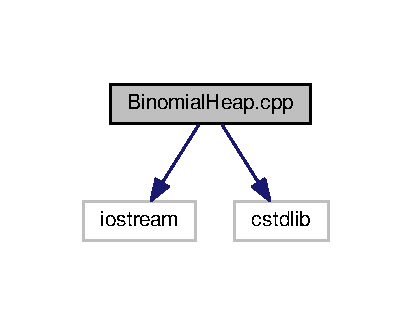
\includegraphics[width=198pt]{BinomialHeap_8cpp__incl}
\end{center}
\end{figure}
\subsection*{Classes}
\begin{DoxyCompactItemize}
\item 
struct \hyperlink{structnode}{node}
\item 
class \hyperlink{classBinomialHeap}{Binomial\+Heap}
\end{DoxyCompactItemize}
\subsection*{Functions}
\begin{DoxyCompactItemize}
\item 
int \hyperlink{BinomialHeap_8cpp_ae66f6b31b5ad750f1fe042a706a4e3d4}{main} ()
\end{DoxyCompactItemize}


\subsection{Function Documentation}
\index{Binomial\+Heap.\+cpp@{Binomial\+Heap.\+cpp}!main@{main}}
\index{main@{main}!Binomial\+Heap.\+cpp@{Binomial\+Heap.\+cpp}}
\subsubsection[{\texorpdfstring{main()}{main()}}]{\setlength{\rightskip}{0pt plus 5cm}int main (
\begin{DoxyParamCaption}
{}
\end{DoxyParamCaption}
)}\hypertarget{BinomialHeap_8cpp_ae66f6b31b5ad750f1fe042a706a4e3d4}{}\label{BinomialHeap_8cpp_ae66f6b31b5ad750f1fe042a706a4e3d4}

\begin{DoxyCode}
332 \{
333     \textcolor{keywordtype}{int} n, m, l, i;
334     \hyperlink{classBinomialHeap}{BinomialHeap} bh;
335     \hyperlink{structnode}{node}* p;
336     \hyperlink{structnode}{node} *H;
337     H = bh.\hyperlink{classBinomialHeap_a3ffaab6756189d14dd76e4e7a48147b6}{Initializeheap}();
338     \textcolor{keywordtype}{char} ch;
339     \textcolor{keywordflow}{while} (1)
340     \{
341         cout<<\textcolor{stringliteral}{"----------------------------"}<<endl;
342         cout<<\textcolor{stringliteral}{"Operations on Binomial heap"}<<endl;
343         cout<<\textcolor{stringliteral}{"----------------------------"}<<endl;
344         cout<<\textcolor{stringliteral}{"1)Insert Element in the heap"}<<endl;
345         cout<<\textcolor{stringliteral}{"2)Extract Minimum key node"}<<endl;
346         cout<<\textcolor{stringliteral}{"3)Decrease key of a node"}<<endl;
347         cout<<\textcolor{stringliteral}{"4)Delete a node"}<<endl;
348         cout<<\textcolor{stringliteral}{"5)Display Heap"}<<endl;
349         cout<<\textcolor{stringliteral}{"6)Exit"}<<endl;
350         cout<<\textcolor{stringliteral}{"Enter Your Choice: "};
351         cin>>l;
352         \textcolor{keywordflow}{switch}(l)
353         \{
354         \textcolor{keywordflow}{case} 1:
355             cout<<\textcolor{stringliteral}{"Enter the element to be inserted: "};
356             cin>>m;
357             p = bh.\hyperlink{classBinomialHeap_a60a7f08bad4dd38fe2b3000d6e29724e}{Create\_node}(m);
358             H = bh.\hyperlink{classBinomialHeap_a762a7e29d6bea85540f1a82cbca4a062}{Insert}(H, p);
359             \textcolor{keywordflow}{break};
360         \textcolor{keywordflow}{case} 2:
361             p = bh.\hyperlink{classBinomialHeap_a71e1468e2782db3f2322d188bca1e48a}{Extract\_Min}(H);
362             \textcolor{keywordflow}{if} (p != NULL)
363                 cout<<\textcolor{stringliteral}{"The node with minimum key: "}<<p->\hyperlink{structnode_a027ad0e5186d6cfab02c74a3da2d28a9}{n}<<endl;
364             \textcolor{keywordflow}{else}
365                 cout<<\textcolor{stringliteral}{"Heap is empty"}<<endl;
366             \textcolor{keywordflow}{break};
367         \textcolor{keywordflow}{case} 3:
368             cout<<\textcolor{stringliteral}{"Enter the key to be decreased: "};
369             cin>>m;
370             cout<<\textcolor{stringliteral}{"Enter new key value: "};
371             cin>>l;
372             bh.\hyperlink{classBinomialHeap_a3898a1fb87677fdb94a40f62ac416de9}{Decrease\_key}(H, m, l);
373             \textcolor{keywordflow}{break};
374         \textcolor{keywordflow}{case} 4:
375             cout<<\textcolor{stringliteral}{"Enter the key to be deleted: "};
376             cin>>m;
377             bh.\hyperlink{classBinomialHeap_aab7ea7e42fe1b2aaf3298f73f4e68884}{Delete}(H, m);
378             \textcolor{keywordflow}{break};
379         \textcolor{keywordflow}{case} 5:
380             cout<<\textcolor{stringliteral}{"The Heap is: "}<<endl;
381             bh.\hyperlink{classBinomialHeap_a43b3339eb8cc6eea26f769ab616b720a}{Display}(H);
382             \textcolor{keywordflow}{break};
383         \textcolor{keywordflow}{case} 6:
384             exit(1);
385         \textcolor{keywordflow}{default}:
386             cout<<\textcolor{stringliteral}{"Wrong Choice"};
387       \}
388     \}
389     \textcolor{keywordflow}{return} 0;
390 \}\end{DoxyCode}


Here is the call graph for this function\+:
\nopagebreak
\begin{figure}[H]
\begin{center}
\leavevmode
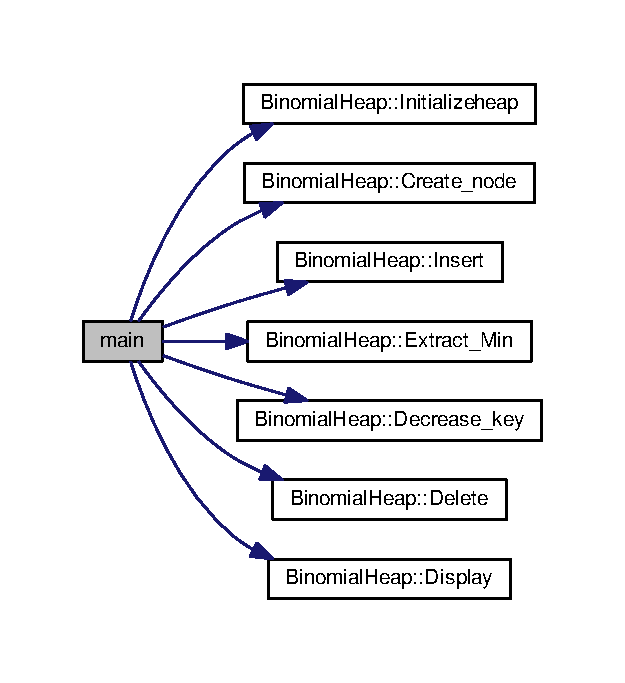
\includegraphics[width=300pt]{BinomialHeap_8cpp_ae66f6b31b5ad750f1fe042a706a4e3d4_cgraph}
\end{center}
\end{figure}



%--- End generated contents ---

% Index
\backmatter
\newpage
\phantomsection
\clearemptydoublepage
\addcontentsline{toc}{chapter}{Index}
\printindex

\end{document}
